\documentclass[10pt,french]{article}

\input preambule_2013
\RegleEntete


\newcommand\competences{
\setcounter{exo}{0}\renewcommand\arraystretch{1.2}
\begin{tabular}{ll} Nom : \\[5pt] Prénom : \end{tabular}
\hfill
\textbf{Note :}
\begin{tabular}{|c|}
\hline
\slashbox{\Huge\bfseries\phantom{10}}{\Huge\bfseries 10}\\
\hline
\end{tabular}\renewcommand\arraystretch{1}
\[***\]
}

\entete{\premiere \stmg}{Tableau de signes \\ Discriminant}{A}
\pieddepage{}{}{}


\begin{document}
\competences

\exo
Calculer le discriminant des polynômes suivants :
\begin{multicols}{3}
\begin{enumerate}
    \item $A(x) = 3x^2 + x - 2$\par\vspace*{5.5cm}
    \item $B(x) = -4x^2 + 3$\par\vspace*{5.5cm}
    \item $C(x) = 1 - 2x^2 + 5x$\par\vspace*{5.5cm}
\end{enumerate}
\end{multicols}
\[*\]

\exo
On considère la fonction $f$ définie pour tout $x \in \R$ par
\[f(x) = -2x^2 + x + 3\]
La courbe représentative de $f$ a été dessinée ci-dessous :

\begin{center}
    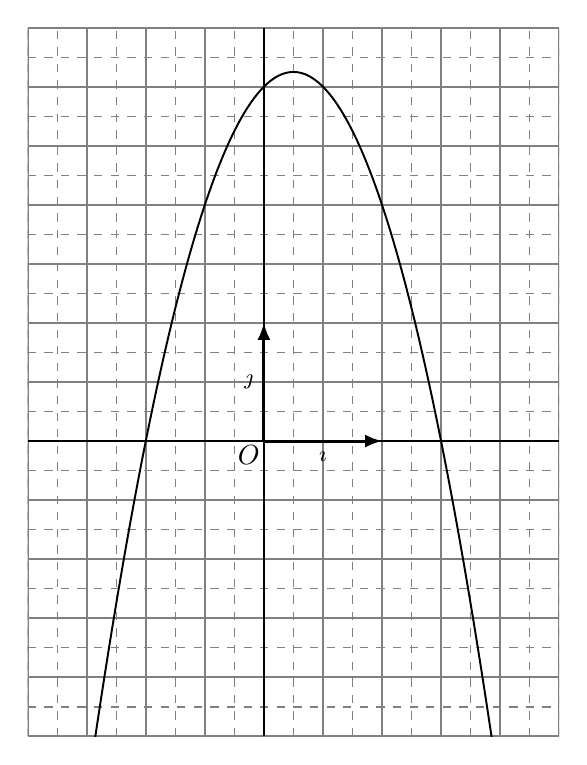
\begin{tikzpicture}[>=latex,scale=0.75,x=2cm,y=2cm]
        \clip (-2,-2.5) rectangle (2.5,3.5);
        \draw[color=white,line width=1pt] plot[domain=-1.5:2,samples=200] (\x,{(-\x-1)*(2*\x-3)});
        \draw[help lines,dashed,line width=0.5pt] (-2,-2.5) grid[step=0.25] (2.5,3.5);
        \draw[help lines,line width=0.7pt] (-2,-2.5) grid[step=0.5] (2.5,3.5);
        \draw[-,line width=1pt] (-2,0) -- (2.5,0); \draw[-,line width=1pt] (0,-2.5) -- (0,3.5);
        \coordinate (O) at (0,0); \draw (O) node[below left = -2pt] {$O$};
        \coordinate (I) at (1,0); \draw[->,line width=1.1pt] (O) -- (I) node[midway,below] {\footnotesize $\vect\imath$};
        \coordinate (J) at (0,1); \draw[->,line width=1.1pt] (O) -- (J) node[midway,left] {\footnotesize $\vect\jmath$};
        \draw[line width=0.7pt] plot[domain=-2:2.5,samples=200] (\x,{-2*(\x)^2+\x+3}) node[right] {$\calig C_f$};
    \end{tikzpicture}
\end{center}

\begin{enumerate}
        \item Résoudre graphiquement l'équation $f(x) = 3$.
        \item Résoudre graphiquement l'inéquation $f(x) \geqslant 2$.
        \item Démontrer que pour tout $x \in \R$, $f(x) = (-x -1)(2x - 3)$.
        \item Par le calcul, résoudre $f(x) = 0$.
        \item À l'aide de la question 3, construire le tableau de signes de la fonction $f$.
        \item À l'aide du tableau de signe, résoudre l'inéquation $f(x) < 0$.
\end{enumerate}

\clearpage

%--------------------------------------------------------------------------------------------------------------------------------------------------------------------------
%                           SUJET B
%--------------------------------------------------------------------------------------------------------------------------------------------------------------------------

\entete{\premiere \stmg}{Tableau de signes \\ Discriminant}{B}
\competences

\exo
Calculer le discriminant des polynômes suivants :
\begin{multicols}{3}
\begin{enumerate}
    \item $A(x) = 2x^2 + x - 4$\par\vspace*{5.5cm}
    \item $B(x) = -3x^2 + 2$\par\vspace*{5.5cm}
    \item $C(x) = 1 - 5x^2 + 3x$\par\vspace*{5.5cm}
\end{enumerate}
\end{multicols}
\[*\]

\exo
On considère la fonction $f$ définie pour tout $x \in \R$ par
\[f(x) = -2x^2 - x + 1\]
La courbe représentative de $f$ a été dessinée ci-dessous :

\begin{center}
    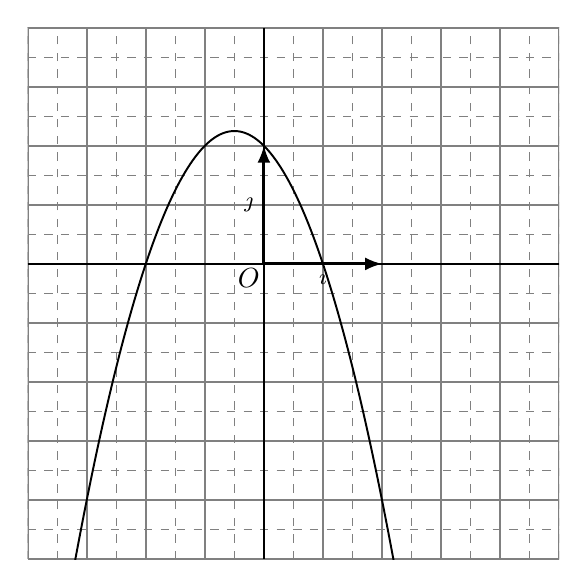
\begin{tikzpicture}[>=latex,scale=0.75,x=2cm,y=2cm]
        \clip (-2,-2.5) rectangle (2.5,2);
        \draw[color=white,line width=1pt] plot[domain=-1.5:2,samples=200] (\x,{(-\x-1)*(2*\x-3)});
        \draw[help lines,dashed,line width=0.5pt] (-2,-2.5) grid[step=0.25] (2.5,3.5);
        \draw[help lines,line width=0.7pt] (-2,-2.5) grid[step=0.5] (2.5,3.5);
        \draw[-,line width=1pt] (-2,0) -- (2.5,0); \draw[-,line width=1pt] (0,-2.5) -- (0,2);
        \coordinate (O) at (0,0); \draw (O) node[below left = -2pt] {$O$};
        \coordinate (I) at (1,0); \draw[->,line width=1.1pt] (O) -- (I) node[midway,below] {\footnotesize $\vect\imath$};
        \coordinate (J) at (0,1); \draw[->,line width=1.1pt] (O) -- (J) node[midway,left] {\footnotesize $\vect\jmath$};
        \draw[line width=0.7pt] plot[domain=-2:2.5,samples=200] (\x,{(-\x-1)*(2*\x-1)}) node[right] {$\calig C_f$};
    \end{tikzpicture}
\end{center}

\begin{enumerate}
        \item Résoudre graphiquement l'équation $f(x) = 1$.
        \item Résoudre graphiquement l'inéquation $f(x) \geqslant -2$.
        \item Démontrer que pour tout $x \in \R$, $f(x) = (-x - 1)(2x - 1)$.
        \item Par le calcul, résoudre $f(x) = 0$.
        \item À l'aide de la question 3, construire le tableau de signes de la fonction $f$.
        \item À l'aide du tableau de signes, résoudre l'inéquation $f(x) < 0$.
\end{enumerate}


\end{document} 